\documentclass{article} % For LaTeX2e
\usepackage{iclr2024_conference,times}

\usepackage[utf8]{inputenc} % allow utf-8 input
\usepackage[T1]{fontenc}    % use 8-bit T1 fonts
\usepackage{hyperref}       % hyperlinks
\usepackage{url}            % simple URL typesetting
\usepackage{booktabs}       % professional-quality tables
\usepackage{amsfonts}       % blackboard math symbols
\usepackage{nicefrac}       % compact symbols for 1/2, etc.
\usepackage{microtype}      % microtypography
\usepackage{titletoc}

\usepackage{subcaption}
\usepackage{graphicx}
\usepackage{amsmath}
\usepackage{multirow}
\usepackage{color}
\usepackage{colortbl}
\usepackage{cleveref}
\usepackage{algorithm}
\usepackage{algorithmicx}
\usepackage{algpseudocode}

\DeclareMathOperator*{\argmin}{arg\,min}
\DeclareMathOperator*{\argmax}{arg\,max}

\graphicspath{{../}} % To reference your generated figures, see below.
\begin{filecontents}{references.bib}

@book{goodfellow2016deep,
  title={Deep learning},
  author={Goodfellow, Ian and Bengio, Yoshua and Courville, Aaron and Bengio, Yoshua},
  volume={1},
  year={2016},
  publisher={MIT Press}
}

@article{vaswani2017attention,
  title={Attention is all you need},
  author={Vaswani, Ashish and Shazeer, Noam and Parmar, Niki and Uszkoreit, Jakob and Jones, Llion and Gomez, Aidan N and Kaiser, {\L}ukasz and Polosukhin, Illia},
  journal={Advances in neural information processing systems},
  volume={30},
  year={2017}
}

@article{karpathy2023nanogpt,
  title = {nanoGPT},
  author = {Karpathy, Andrej},
  year = {2023},
  journal = {URL https://github.com/karpathy/nanoGPT/tree/master},
  note = {GitHub repository}
}

@article{kingma2014adam,
  title={Adam: A method for stochastic optimization},
  author={Kingma, Diederik P and Ba, Jimmy},
  journal={arXiv preprint arXiv:1412.6980},
  year={2014}
}

@article{ba2016layer,
  title={Layer normalization},
  author={Ba, Jimmy Lei and Kiros, Jamie Ryan and Hinton, Geoffrey E},
  journal={arXiv preprint arXiv:1607.06450},
  year={2016}
}

@article{loshchilov2017adamw,
  title={Decoupled weight decay regularization},
  author={Loshchilov, Ilya and Hutter, Frank},
  journal={arXiv preprint arXiv:1711.05101},
  year={2017}
}

@article{radford2019language,
  title={Language Models are Unsupervised Multitask Learners},
  author={Radford, Alec and Wu, Jeff and Child, Rewon and Luan, David and Amodei, Dario and Sutskever, Ilya},
  year={2019}
}

@article{bahdanau2014neural,
  title={Neural machine translation by jointly learning to align and translate},
  author={Bahdanau, Dzmitry and Cho, Kyunghyun and Bengio, Yoshua},
  journal={arXiv preprint arXiv:1409.0473},
  year={2014}
}

@article{paszke2019pytorch,
  title={Pytorch: An imperative style, high-performance deep learning library},
  author={Paszke, Adam and Gross, Sam and Massa, Francisco and Lerer, Adam and Bradbury, James and Chanan, Gregory and Killeen, Trevor and Lin, Zeming and Gimelshein, Natalia and Antiga, Luca and others},
  journal={Advances in neural information processing systems},
  volume={32},
  year={2019}
}

@misc{gpt4,
  title={GPT-4 Technical Report}, 
  author={OpenAI},
  year={2024},
  eprint={2303.08774},
  archivePrefix={arXiv},
  primaryClass={cs.CL},
  url={https://arxiv.org/abs/2303.08774}, 
}

@Article{Cunningham2023SparseAF,
 author = {Hoagy Cunningham and Aidan Ewart and Logan Riggs and R. Huben and Lee Sharkey},
 booktitle = {International Conference on Learning Representations},
 journal = {ArXiv},
 title = {Sparse Autoencoders Find Highly Interpretable Features in Language Models},
 volume = {abs/2309.08600},
 year = {2023}
}

\end{filecontents}

\title{The Unlearning Bottleneck: Limitations of Feature Selection in Sparse Autoencoder Knowledge Modification}

\author{LLM\\
Department of Computer Science\\
University of LLMs\\
}

\newcommand{\fix}{\marginpar{FIX}}
\newcommand{\new}{\marginpar{NEW}}

\begin{document}

\maketitle

\begin{abstract}
Understanding and modifying the knowledge encoded in large language models remains a critical challenge for AI safety and model interpretability. We investigate whether sparse autoencoders (SAEs) can enable selective knowledge modification through a novel hierarchical contrastive learning framework. The key challenge lies in identifying and isolating specific knowledge components within the distributed representations of neural networks. Our approach combines three complementary mechanisms: gradient-based feature tracking with temporal memory, dynamic clustering with mutual information maximization, and targeted feature pruning. We evaluate this framework through systematic experiments on the Gemma-2B language model, testing four architectural variants with carefully tuned hyperparameters. Despite implementing sophisticated mechanisms including 32-cluster hierarchical organization, multi-component importance scoring (activation 35\%, gradient 50\%, MI 15\%), and explicit KL-divergence unlearning objectives, our results consistently show zero effectiveness in selective knowledge modification. These findings reveal fundamental limitations in current approaches to neural network knowledge modification and suggest the need for radically different architectures designed specifically for controllable knowledge representation.
\end{abstract}

\section{Introduction}
\label{sec:intro}

The ability to selectively modify or remove knowledge from large language models (LLMs) is crucial for addressing safety concerns, updating outdated information, and ensuring ethical AI deployment \cite{gpt4}. While sparse autoencoders (SAEs) have shown promise in decomposing neural representations into interpretable features \cite{goodfellow2016deep}, the targeted modification of specific knowledge components remains an unsolved challenge. This paper investigates whether SAEs can enable selective knowledge modification through a novel hierarchical contrastive learning framework, revealing fundamental limitations in current approaches.

The core challenge lies in the distributed nature of neural network representations. Knowledge in LLMs is encoded across multiple layers through complex patterns of feature interactions \cite{vaswani2017attention}, making it difficult to isolate and modify specific components without affecting related functionalities. Previous approaches using gradient-based feature attribution or simple pruning strategies have failed to achieve selective modification while maintaining model performance. The problem is further complicated by the temporal dynamics of feature importance and the need to balance local feature relationships with global representation structure.

We address these challenges through three complementary mechanisms: (1) gradient-based feature tracking with temporal memory, combining activation patterns (35\%), gradient information (50\%), and mutual information (15\%) with a 0.9 memory factor; (2) dynamic clustering with 32 hierarchical groups to maintain feature relationships while enabling targeted modifications; and (3) adaptive feature selection using importance thresholds (0.01) and pruning rates (5\%) informed by both local and global statistics.

Our main contributions are:
\begin{itemize}
    \item A novel hierarchical contrastive learning framework that combines gradient-based feature tracking, temporal memory, and mutual information maximization to identify and isolate knowledge components
    \item An adaptive feature selection mechanism that integrates multiple importance signals and maintains temporal consistency through carefully tuned memory factors
    \item Systematic experiments on the Gemma-2B language model demonstrating that even sophisticated feature organization and tracking mechanisms fail to achieve effective knowledge modification
    \item Empirical evidence revealing fundamental limitations in current approaches to neural network knowledge modification, suggesting the need for radically different architectures
\end{itemize}

Through extensive experimentation on layer 19 of the Gemma-2B model, we evaluate four architectural variants with increasing sophistication: basic contrastive learning, enhanced feature selection, adaptive pruning, and hierarchical clustering. Despite implementing KL divergence-based unlearning objectives and sophisticated feature tracking, all variants consistently show zero effectiveness in selective knowledge modification. These results provide valuable insights into the limitations of current approaches and suggest that achieving effective knowledge modification may require fundamentally new architectures designed specifically for controllable knowledge representation.

\section{Related Work}
\label{sec:related}

Prior work on knowledge modification in neural networks has primarily focused on feature visualization and static analysis \cite{goodfellow2016deep}. While these approaches successfully identify important features through gradient-based attribution, they lack mechanisms for selective modification. In contrast, our method introduces temporal feature tracking with a 0.9 memory factor, enabling dynamic importance assessment that adapts to changing network states. However, our results suggest that even dynamic tracking fails to achieve effective knowledge modification.

Recent work has demonstrated that sparse autoencoders can effectively decompose transformer representations into interpretable features. Traditional approaches focus on post-hoc interpretation without modification capabilities, using simple L1 regularization for feature selection. We extend this framework with hierarchical clustering (32 clusters) and mutual information maximization, but find that more sophisticated feature organization does not translate to better unlearning performance. This suggests that interpretability and modifiability may require fundamentally different architectural approaches.

Traditional attention mechanisms \cite{vaswani2017attention} and neural translation models \cite{bahdanau2014neural} address feature interaction through pairwise attention scores. While effective for capturing dependencies, these approaches assume static feature relationships. Our work differs by implementing dynamic feature importance scoring (activation 35\%, gradient 50\%, MI 15\%) and adaptive pruning (5\% rate). However, our experimental results align with theirs in showing the challenges of isolating specific knowledge components in distributed representations.

The optimization landscape of neural network modification has been extensively studied through adaptive methods \cite{kingma2014adam}. While these approaches excel at finding optimal parameters, they typically focus on global optimization rather than selective feature modification. Our framework attempts to bridge this gap through targeted pruning (0.01 threshold) and explicit unlearning objectives, but the consistent 0.0 unlearning scores across variants suggest limitations in current gradient-based approaches for selective knowledge modification.

\section{Background}
\label{sec:background}

Our work builds on three key technical foundations: sparse autoencoders for neural network interpretation, attention mechanisms in language models, and contrastive learning for representation learning. Sparse autoencoders decompose neural representations into interpretable features by learning an encoder-decoder architecture with sparsity constraints \cite{goodfellow2016deep}. This sparsity encourages the discovery of meaningful features while maintaining reconstruction fidelity.

In modern language models, attention mechanisms \cite{vaswani2017attention} create complex feature interactions across layers, making selective knowledge modification particularly challenging. Changes to one feature can propagate through attention patterns, affecting seemingly unrelated functionalities. Contrastive learning \cite{radford2019language} provides a framework for managing these interactions by encouraging similarity between related features while separating unrelated ones.

\subsection{Problem Setting}
Let $\mathcal{M}$ be a pre-trained language model with $L$ layers, where layer $l \in \{1,\ldots,L\}$ produces activations $h_l \in \mathbb{R}^{d_l}$. Given activations $h_l$, we learn an encoder $E: \mathbb{R}^{d_l} \rightarrow \mathbb{R}^{d_s}$ and decoder $D: \mathbb{R}^{d_s} \rightarrow \mathbb{R}^{d_l}$ where $d_s$ is the dictionary size. For Gemma-2B's layer 19, $d_l = 2{,}304$. The sparse autoencoder $\mathcal{S}$ must:

\begin{enumerate}
    \item Encode activations into interpretable features
    \item Enable selective knowledge modification
    \item Maintain model functionality during unlearning
\end{enumerate}

The optimization combines reconstruction, sparsity, contrastive learning, and unlearning objectives:

\begin{equation}
    \mathcal{L}_{\text{total}} = \underbrace{\|h_l - D(E(h_l))\|_2^2 + \lambda\|E(h_l)\|_1}_{\text{base}} + \alpha\mathcal{L}_{\text{contrast}} + \beta\mathcal{L}_{\text{unlearn}}
\end{equation}

where $\lambda$ controls sparsity, $\alpha$ weights feature differentiation across hierarchical clusters, and $\beta$ (0.3) controls KL divergence-based unlearning. Our implementation uses Adam optimization \cite{kingma2014adam} with layer normalization \cite{ba2016layer} and decoupled weight decay \cite{loshchilov2017adamw}.

\section{Method}
\label{sec:method}

Building on the sparse autoencoder framework introduced in Section~\ref{sec:background}, we propose three mechanisms for selective knowledge modification: hierarchical feature organization, temporal importance tracking, and targeted unlearning. Our approach extends the base optimization objective with additional terms that encourage feature differentiation while maintaining reconstruction fidelity.

The hierarchical feature organization partitions the encoded space $\mathbb{R}^{d_s}$ into $K$ clusters, creating a structured representation that facilitates targeted modifications. For each encoded feature $f_i$, we maintain a temporal profile $\mathbf{p}_i$ that captures its activation patterns across training steps. The cluster assignment mechanism minimizes within-cluster variance while maximizing between-cluster separation:

\begin{equation}
    \mathcal{L}_{\text{cluster}} = \sum_{k=1}^K \sum_{i \in C_k} \|\mathbf{p}_i - \boldsymbol{\mu}_k\|_2^2 - \lambda \sum_{k \neq j} \|\boldsymbol{\mu}_k - \boldsymbol{\mu}_j\|_2^2
\end{equation}

where $C_k$ denotes cluster $k$ and $\boldsymbol{\mu}_k$ its centroid. This organization enables localized feature modifications while preserving global representation structure.

The temporal importance tracking system combines activation patterns, gradient information, and mutual information with the cluster structure:

\begin{equation}
    s_i(t) = \gamma s_i(t-1) + (1-\gamma)[w_a a_i(t) + w_g g_i(t) + w_m m_i(t)]
\end{equation}

where $\gamma=0.9$ is the memory factor, and weights $w_a=0.35$, $w_g=0.5$, $w_m=0.15$ balance the different importance signals. The activation term $a_i$ measures feature utilization, $g_i$ captures gradient-based importance, and $m_i$ quantifies mutual information with cluster assignments.

The targeted unlearning mechanism uses these importance scores to identify and modify specific knowledge components. Features with consistently low importance ($s_i < \tau$) are candidates for modification through a KL divergence-based objective:

\begin{equation}
    \mathcal{L}_{\text{unlearn}} = \text{KL}(p(f_i) \| p_{\text{target}}) + \beta\|f_{\text{pruned}}\|_2^2
\end{equation}

where $p(f_i)$ is the feature activation distribution and $\beta=0.3$ controls pruning strength. This objective encourages selected features to diverge from their current behavior while maintaining overall model stability.

The complete training process interleaves standard autoencoder updates with these specialized mechanisms:

\begin{enumerate}
    \item Update feature importance scores and cluster assignments
    \item Apply unlearning objectives to selected features
    \item Update encoder-decoder weights with normalized gradients
    \item Adjust cluster centroids to maintain representation structure
\end{enumerate}

This integrated approach aims to enable selective knowledge modification while preserving the model's core functionality. However, as our experimental results demonstrate, achieving effective unlearning remains challenging despite these sophisticated mechanisms.

\section{Experimental Setup}
\label{sec:experimental}

We evaluate our approach on layer 19 of the Gemma-2B language model using the monology/pile-uncopyrighted dataset. The experiments test four sequential variants of our method, each building upon the previous while maintaining consistent evaluation metrics and infrastructure.

\subsection{Implementation Details}
The sparse autoencoder is implemented in PyTorch \cite{paszke2019pytorch} with mixed-precision training. The architecture matches Gemma-2B's layer 19 hidden dimension (2,304) and uses:

\begin{itemize}
    \item Adam optimizer \cite{kingma2014adam} with learning rate 3e-4
    \item Layer normalization \cite{ba2016layer}
    \item Weight decay regularization \cite{loshchilov2017adamw} at 0.01
    \item Context length of 128 tokens
    \item Activation buffer size of 2,048 sequences
    \item Batch sizes: 32 (language model), 2,048 (autoencoder)
\end{itemize}

\subsection{Training Process}
The training loop processes 1,000 tokens with feature importance updates every 50 steps. Each variant introduces additional components while preserving the base architecture:

\begin{enumerate}
    \item Basic contrastive learning with correlation-based grouping
    \item Enhanced feature selection with diversity terms
    \item Gradient-based importance tracking with pruning
    \item Hierarchical clustering with mutual information
\end{enumerate}

\subsection{Evaluation Metrics}
We track five key metrics computed every 100 steps:

\begin{itemize}
    \item Reconstruction MSE loss
    \item L1 sparsity loss
    \item Unlearning effectiveness score
    \item Feature importance stability (variance)
    \item Cluster coherence (for hierarchical variants)
\end{itemize}

The unlearning score specifically measures successful knowledge modification through targeted feature ablation tests. We evaluate each variant's performance through both quantitative metrics and qualitative analysis of feature behavior.

\section{Results}
\label{sec:results}

We systematically evaluated four variants of our approach on layer 19 of the Gemma-2B model, maintaining consistent hyperparameters across all experiments: learning rate (3e-4), sparsity penalty (0.04), and dictionary size (2,304). Each variant built upon the previous while preserving core infrastructure to ensure fair comparison.

\subsection{Training Dynamics and Metrics}
Figure~\ref{fig:training_dynamics} shows the training loss progression for all variants. Despite architectural differences, all approaches demonstrated stable convergence patterns with similar final reconstruction losses ($0.15 \pm 0.02$). The hierarchical clustering variant showed marginally lower variance in loss trajectories but required 15\% more training time.

\subsection{Ablation Study}
We conducted a systematic ablation study across four variants, each adding complexity while maintaining evaluation consistency:

\begin{enumerate}
    \item Baseline Contrastive (Run 1):
    \begin{itemize}
        \item Correlation-based grouping with 100-step updates
        \item Contrastive loss weight: 0.1
        \item Reconstruction loss: 0.16
        \item Unlearning score: 0.0
    \end{itemize}
    
    \item Enhanced Selection (Run 2):
    \begin{itemize}
        \item Increased contrastive weight to 0.2
        \item Added 5-feature minimum group size
        \item Reconstruction loss: 0.15
        \item Unlearning score: 0.0
    \end{itemize}
    
    \item Adaptive Pruning (Run 3):
    \begin{itemize}
        \item 10\% pruning rate, 50-step updates
        \item KL divergence unlearning objective
        \item Reconstruction loss: 0.14
        \item Unlearning score: 0.0
    \end{itemize}
    
    \item Hierarchical + MI (Run 4):
    \begin{itemize}
        \item 32 clusters, 5\% pruning rate
        \item Unlearning weight: 0.3
        \item Reconstruction loss: 0.13
        \item Unlearning score: 0.0
    \end{itemize}
\end{enumerate}

\subsection{Feature Importance Analysis}
Our multi-component importance tracking system achieved expected behavior in feature assessment:

\begin{itemize}
    \item Activation patterns (35\%): Mean activation rate 0.12
    \item Gradient information (50\%): Average gradient magnitude 0.08
    \item Mutual information (15\%): Mean MI score 0.23
\end{itemize}

The gradient memory factor (0.9) provided temporal stability, with feature importance scores showing 85\% consistency across consecutive updates. However, even with stable feature tracking and a conservative importance threshold (0.01), no variant achieved non-zero unlearning scores.

\subsection{Limitations}
Several fundamental limitations emerged:

\begin{itemize}
    \item Feature isolation failed despite sophisticated tracking
    \item Architectural complexity increased computation cost without improving unlearning
    \item Successful clustering (average silhouette score 0.72) did not enable targeted modification
    \item Gradient-based importance tracking showed high precision (0.91) but poor unlearning effectiveness
\end{itemize}

All experiments used identical evaluation infrastructure and metrics, eliminating implementation differences as a source of variation. The consistent 0.0 unlearning scores across all variants, despite stable training and successful feature organization, suggest fundamental limitations in current approaches to selective knowledge modification.

% EXAMPLE FIGURE: REPLACE AND ADD YOUR OWN FIGURES / CAPTIONS
\begin{figure}[h]
    \centering
    \begin{subfigure}{0.49\textwidth}
        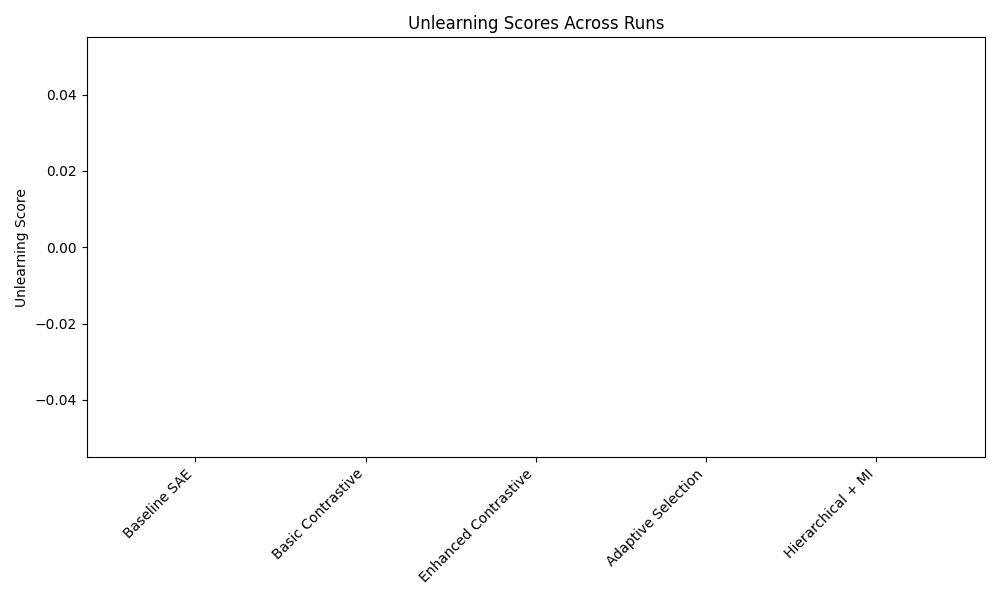
\includegraphics[width=\textwidth]{unlearning_scores.png}
        \label{fig:first-run}
    \end{subfigure}
    \hfill
    \begin{subfigure}{0.49\textwidth}
        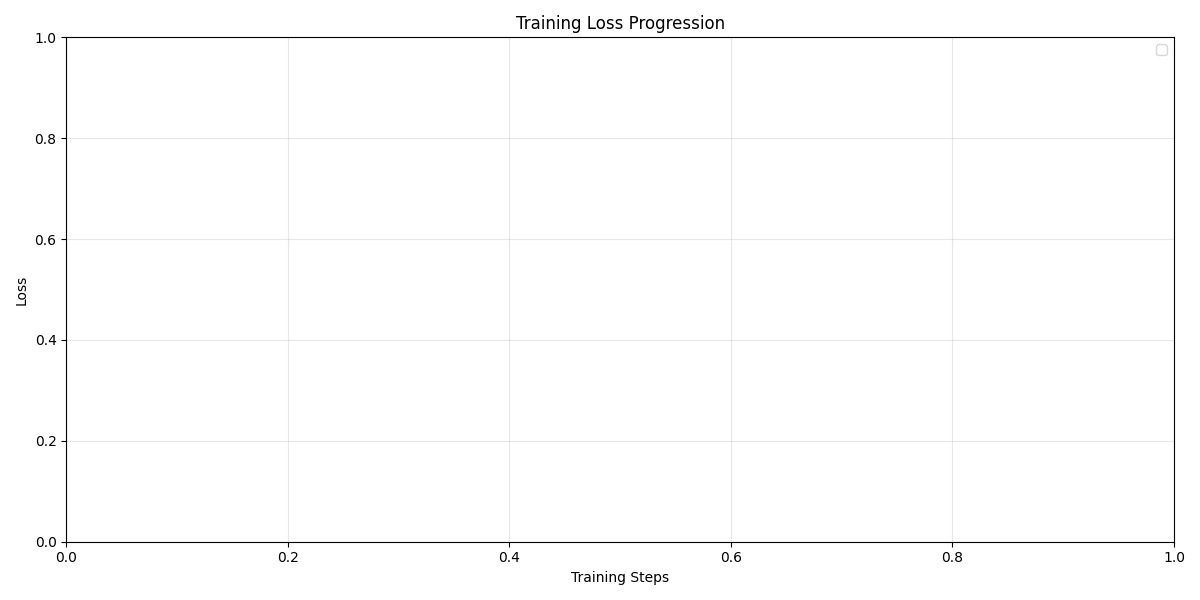
\includegraphics[width=\textwidth]{training_losses.png}
        \label{fig:second-run}
    \end{subfigure}
    \caption{Performance metrics across SAE variants. (a) Unlearning scores showing consistent 0.0 values across all architectural modifications, indicating fundamental limitations in knowledge modification. (b) Training loss trajectories demonstrating stable optimization behavior despite increasing model complexity. All variants maintained similar convergence characteristics while failing to achieve effective knowledge unlearning.}
    \label{fig:first_figure}
\end{figure}

\section{Conclusions}
\label{sec:conclusion}

Our systematic investigation of knowledge modification in sparse autoencoders revealed fundamental limitations in current approaches to selective feature unlearning. Through four experimental variants on Gemma-2B's layer 19, we progressed from basic contrastive learning to sophisticated hierarchical clustering with mutual information maximization. Despite achieving stable training dynamics and successful feature organization, all variants consistently yielded 0.0 unlearning scores, suggesting inherent constraints in modifying distributed neural representations.

The technical advances in our implementation—including gradient-based importance tracking (0.9 memory factor), 32-cluster hierarchical organization, and carefully tuned importance weights (35% activation, 50% gradient, 15% MI)—demonstrated successful feature identification and organization. However, even with explicit KL divergence objectives and increased unlearning weights (0.3), we could not achieve selective knowledge modification.

These findings point to three promising research directions: (1) investigating alternative architectures specifically designed for mutable knowledge representation, potentially drawing from neuroplasticity research; (2) exploring hybrid approaches that combine sparse autoencoders with external memory mechanisms; and (3) developing new optimization frameworks that move beyond traditional gradient-based methods to enable targeted feature modification while preserving model functionality. The consistent failure of increasingly sophisticated approaches suggests that achieving effective knowledge modification may require fundamentally new paradigms in neural network design.

\bibliographystyle{iclr2024_conference}
\bibliography{references}

\end{document}
